\documentclass[1p]{elsarticle_modified}
%\bibliographystyle{elsarticle-num}

%\usepackage[colorlinks]{hyperref}
%\usepackage{abbrmath_seonhwa} %\Abb, \Ascr, \Acal ,\Abf, \Afrak
\usepackage{amsfonts}
\usepackage{amssymb}
\usepackage{amsmath}
\usepackage{amsthm}
\usepackage{scalefnt}
\usepackage{amsbsy}
\usepackage{kotex}
\usepackage{caption}
\usepackage{subfig}
\usepackage{color}
\usepackage{graphicx}
\usepackage{xcolor} %% white, black, red, green, blue, cyan, magenta, yellow
\usepackage{float}
\usepackage{setspace}
\usepackage{hyperref}

\usepackage{tikz}
\usetikzlibrary{arrows}

\usepackage{multirow}
\usepackage{array} % fixed length table
\usepackage{hhline}

%%%%%%%%%%%%%%%%%%%%%
\makeatletter
\renewcommand*\env@matrix[1][\arraystretch]{%
	\edef\arraystretch{#1}%
	\hskip -\arraycolsep
	\let\@ifnextchar\new@ifnextchar
	\array{*\c@MaxMatrixCols c}}
\makeatother %https://tex.stackexchange.com/questions/14071/how-can-i-increase-the-line-spacing-in-a-matrix
%%%%%%%%%%%%%%%

\usepackage[normalem]{ulem}

\newcommand{\msout}[1]{\ifmmode\text{\sout{\ensuremath{#1}}}\else\sout{#1}\fi}
%SOURCE: \msout is \stkout macro in https://tex.stackexchange.com/questions/20609/strikeout-in-math-mode

\newcommand{\cancel}[1]{
	\ifmmode
	{\color{red}\msout{#1}}
	\else
	{\color{red}\sout{#1}}
	\fi
}

\newcommand{\add}[1]{
	{\color{blue}\uwave{#1}}
}

\newcommand{\replace}[2]{
	\ifmmode
	{\color{red}\msout{#1}}{\color{blue}\uwave{#2}}
	\else
	{\color{red}\sout{#1}}{\color{blue}\uwave{#2}}
	\fi
}

\newcommand{\Sol}{\mathcal{S}} %segment
\newcommand{\D}{D} %diagram
\newcommand{\A}{\mathcal{A}} %arc


%%%%%%%%%%%%%%%%%%%%%%%%%%%%%5 test

\def\sl{\operatorname{\textup{SL}}(2,\Cbb)}
\def\psl{\operatorname{\textup{PSL}}(2,\Cbb)}
\def\quan{\mkern 1mu \triangleright \mkern 1mu}

\theoremstyle{definition}
\newtheorem{thm}{Theorem}[section]
\newtheorem{prop}[thm]{Proposition}
\newtheorem{lem}[thm]{Lemma}
\newtheorem{ques}[thm]{Question}
\newtheorem{cor}[thm]{Corollary}
\newtheorem{defn}[thm]{Definition}
\newtheorem{exam}[thm]{Example}
\newtheorem{rmk}[thm]{Remark}
\newtheorem{alg}[thm]{Algorithm}

\newcommand{\I}{\sqrt{-1}}
\begin{document}

%\begin{frontmatter}
%
%\title{Boundary parabolic representations of knots up to 8 crossings}
%
%%% Group authors per affiliation:
%\author{Yunhi Cho} 
%\address{Department of Mathematics, University of Seoul, Seoul, Korea}
%\ead{yhcho@uos.ac.kr}
%
%
%\author{Seonhwa Kim} %\fnref{s_kim}}
%\address{Center for Geometry and Physics, Institute for Basic Science, Pohang, 37673, Korea}
%\ead{ryeona17@ibs.re.kr}
%
%\author{Hyuk Kim}
%\address{Department of Mathematical Sciences, Seoul National University, Seoul 08826, Korea}
%\ead{hyukkim@snu.ac.kr}
%
%\author{Seokbeom Yoon}
%\address{Department of Mathematical Sciences, Seoul National University, Seoul, 08826,  Korea}
%\ead{sbyoon15@snu.ac.kr}
%
%\begin{abstract}
%We find all boundary parabolic representation of knots up to 8 crossings.
%
%\end{abstract}
%\begin{keyword}
%    \MSC[2010] 57M25 
%\end{keyword}
%
%\end{frontmatter}

%\linenumbers
%\tableofcontents
%
\newcommand\colored[1]{\textcolor{white}{\rule[-0.35ex]{0.8em}{1.4ex}}\kern-0.8em\color{red} #1}%
%\newcommand\colored[1]{\textcolor{white}{ #1}\kern-2.17ex	\textcolor{white}{ #1}\kern-1.81ex	\textcolor{white}{ #1}\kern-2.15ex\color{red}#1	}

{\Large $\underline{12n_{0111}~(K12n_{0111})}$}

\setlength{\tabcolsep}{10pt}
\renewcommand{\arraystretch}{1.6}
\vspace{1cm}\begin{tabular}{m{100pt}>{\centering\arraybackslash}m{274pt}}
\multirow{5}{120pt}{
	\centering
	\includegraphics[width=112pt]{../../../GIT/diagram.site/Diagrams/png/2200_12n_0111.png}\\
\ \ \ A knot diagram\footnotemark}&
\allowdisplaybreaks
\textbf{Linearized knot diagam} \\
\cline{2-2}
 &
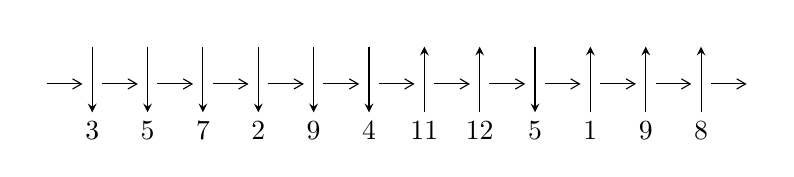
\begin{tikzpicture}[x=20pt, y=17pt]
	% nodes
	\node (C0) at (0, 0) {};
	\node (C1) at (1, 0) {};
	\node (C1U) at (1, +1) {};
	\node (C1D) at (1, -1) {3};

	\node (C2) at (2, 0) {};
	\node (C2U) at (2, +1) {};
	\node (C2D) at (2, -1) {5};

	\node (C3) at (3, 0) {};
	\node (C3U) at (3, +1) {};
	\node (C3D) at (3, -1) {7};

	\node (C4) at (4, 0) {};
	\node (C4U) at (4, +1) {};
	\node (C4D) at (4, -1) {2};

	\node (C5) at (5, 0) {};
	\node (C5U) at (5, +1) {};
	\node (C5D) at (5, -1) {9};

	\node (C6) at (6, 0) {};
	\node (C6U) at (6, +1) {};
	\node (C6D) at (6, -1) {4};

	\node (C7) at (7, 0) {};
	\node (C7U) at (7, +1) {};
	\node (C7D) at (7, -1) {11};

	\node (C8) at (8, 0) {};
	\node (C8U) at (8, +1) {};
	\node (C8D) at (8, -1) {12};

	\node (C9) at (9, 0) {};
	\node (C9U) at (9, +1) {};
	\node (C9D) at (9, -1) {5};

	\node (C10) at (10, 0) {};
	\node (C10U) at (10, +1) {};
	\node (C10D) at (10, -1) {1};

	\node (C11) at (11, 0) {};
	\node (C11U) at (11, +1) {};
	\node (C11D) at (11, -1) {9};

	\node (C12) at (12, 0) {};
	\node (C12U) at (12, +1) {};
	\node (C12D) at (12, -1) {8};
	\node (C13) at (13, 0) {};

	% arrows
	\draw[->,>={angle 60}]
	(C0) edge (C1) (C1) edge (C2) (C2) edge (C3) (C3) edge (C4) (C4) edge (C5) (C5) edge (C6) (C6) edge (C7) (C7) edge (C8) (C8) edge (C9) (C9) edge (C10) (C10) edge (C11) (C11) edge (C12) (C12) edge (C13) ;	\draw[->,>=stealth]
	(C1U) edge (C1D) (C2U) edge (C2D) (C3U) edge (C3D) (C4U) edge (C4D) (C5U) edge (C5D) (C6U) edge (C6D) (C7D) edge (C7U) (C8D) edge (C8U) (C9U) edge (C9D) (C10D) edge (C10U) (C11D) edge (C11U) (C12D) edge (C12U) ;
	\end{tikzpicture} \\
\hhline{~~} \\& 
\textbf{Solving Sequence} \\ \cline{2-2} 
 &
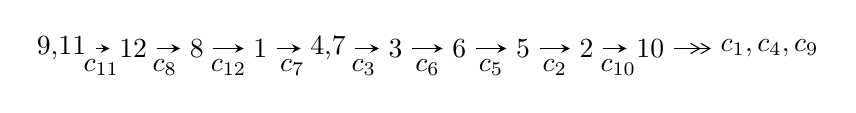
\begin{tikzpicture}[x=23pt, y=7pt]
	% node
	\node (A0) at (-1/8, 0) {9,11};
	\node (A1) at (1, 0) {12};
	\node (A2) at (2, 0) {8};
	\node (A3) at (3, 0) {1};
	\node (A4) at (65/16, 0) {4,7};
	\node (A5) at (41/8, 0) {3};
	\node (A6) at (49/8, 0) {6};
	\node (A7) at (57/8, 0) {5};
	\node (A8) at (65/8, 0) {2};
	\node (A9) at (73/8, 0) {10};
	\node (C1) at (1/2, -1) {$c_{11}$};
	\node (C2) at (3/2, -1) {$c_{8}$};
	\node (C3) at (5/2, -1) {$c_{12}$};
	\node (C4) at (7/2, -1) {$c_{7}$};
	\node (C5) at (37/8, -1) {$c_{3}$};
	\node (C6) at (45/8, -1) {$c_{6}$};
	\node (C7) at (53/8, -1) {$c_{5}$};
	\node (C8) at (61/8, -1) {$c_{2}$};
	\node (C9) at (69/8, -1) {$c_{10}$};
	\node (A10) at (11, 0) {$c_{1},c_{4},c_{9}$};

	% edge
	\draw[->,>=stealth]	
	(A0) edge (A1) (A1) edge (A2) (A2) edge (A3) (A3) edge (A4) (A4) edge (A5) (A5) edge (A6) (A6) edge (A7) (A7) edge (A8) (A8) edge (A9) ;
	\draw[->>,>={angle 60}]	
	(A9) edge (A10);
\end{tikzpicture} \\ 

\end{tabular} \\

\footnotetext{
The image of knot diagram is generated by the software ``\textbf{Draw programme}" developed by Andrew Bartholomew(\url{http://www.layer8.co.uk/maths/draw/index.htm\#Running-draw}), where we modified some parts for our purpose(\url{https://github.com/CATsTAILs/LinksPainter}).
}\phantom \\ \newline 
\centering \textbf{Ideals for irreducible components\footnotemark of $X_{\text{par}}$} 
 
\begin{align*}
I^u_{1}&=\langle 
-1.05669\times10^{17} u^{53}-3.57059\times10^{17} u^{52}+\cdots+7.54024\times10^{16} b+4.04284\times10^{16},\\
\phantom{I^u_{1}}&\phantom{= \langle  }1.02527\times10^{17} u^{53}+3.61000\times10^{17} u^{52}+\cdots+7.54024\times10^{16} a-5.95597\times10^{17},\;u^{54}+4 u^{53}+\cdots-13 u-1\rangle \\
I^u_{2}&=\langle 
a u- u^2+b+a,\;- u^2 a+a^2+1,\;u^3- u^2+2 u-1\rangle \\
I^u_{3}&=\langle 
u^2+b+u,\;- u^2+a-2,\;u^3- u^2+2 u-1\rangle \\
\\
\end{align*}
\raggedright * 3 irreducible components of $\dim_{\mathbb{C}}=0$, with total 63 representations.\\
\footnotetext{All coefficients of polynomials are rational numbers. But the coefficients are sometimes approximated in decimal forms when there is not enough margin.}
\newpage
\renewcommand{\arraystretch}{1}
\centering \section*{I. $I^u_{1}= \langle -1.06\times10^{17} u^{53}-3.57\times10^{17} u^{52}+\cdots+7.54\times10^{16} b+4.04\times10^{16},\;1.03\times10^{17} u^{53}+3.61\times10^{17} u^{52}+\cdots+7.54\times10^{16} a-5.96\times10^{17},\;u^{54}+4 u^{53}+\cdots-13 u-1 \rangle$}
\flushleft \textbf{(i) Arc colorings}\\
\begin{tabular}{m{7pt} m{180pt} m{7pt} m{180pt} }
\flushright $a_{9}=$&$\begin{pmatrix}0\\u\end{pmatrix}$ \\
\flushright $a_{11}=$&$\begin{pmatrix}1\\0\end{pmatrix}$ \\
\flushright $a_{12}=$&$\begin{pmatrix}1\\- u^2\end{pmatrix}$ \\
\flushright $a_{8}=$&$\begin{pmatrix}- u\\u^3+u\end{pmatrix}$ \\
\flushright $a_{1}=$&$\begin{pmatrix}u^2+1\\- u^4-2 u^2\end{pmatrix}$ \\
\flushright $a_{4}=$&$\begin{pmatrix}-1.35974 u^{53}-4.78764 u^{52}+\cdots+20.4946 u+7.89891\\1.40141 u^{53}+4.73538 u^{52}+\cdots-10.6807 u-0.536168\end{pmatrix}$ \\
\flushright $a_{7}=$&$\begin{pmatrix}- u^3-2 u\\u^3+u\end{pmatrix}$ \\
\flushright $a_{3}=$&$\begin{pmatrix}0.267734 u^{53}+0.167743 u^{52}+\cdots+2.48003 u+6.45689\\-0.218764 u^{53}-0.990227 u^{52}+\cdots+3.51913 u+0.584554\end{pmatrix}$ \\
\flushright $a_{6}=$&$\begin{pmatrix}0.166746 u^{53}+0.935589 u^{52}+\cdots-14.0641 u-4.81630\\0.693852 u^{53}+2.26828 u^{52}+\cdots-3.45221 u-0.695131\end{pmatrix}$ \\
\flushright $a_{5}=$&$\begin{pmatrix}0.166746 u^{53}+0.935589 u^{52}+\cdots-14.0641 u-4.81630\\0.629304 u^{53}+2.35002 u^{52}+\cdots-7.11080 u-0.963735\end{pmatrix}$ \\
\flushright $a_{2}=$&$\begin{pmatrix}-1.06576 u^{53}-3.70343 u^{52}+\cdots+13.6083 u+5.08949\\0.272628 u^{53}+0.559742 u^{52}+\cdots+6.49074 u+0.762024\end{pmatrix}$ \\
\flushright $a_{10}=$&$\begin{pmatrix}- u^6-3 u^4-2 u^2+1\\u^8+4 u^6+4 u^4\end{pmatrix}$\\&\end{tabular}
\flushleft \textbf{(ii) Obstruction class $= -1$}\\~\\
\flushleft \textbf{(iii) Cusp Shapes $= \frac{26029323830005351}{12567067818736266} u^{53}+\frac{97584229084765271}{12567067818736266} u^{52}+\cdots-\frac{1438600135913750963}{25134135637472532} u-\frac{393297976137728599}{25134135637472532}$}\\~\\
\newpage\renewcommand{\arraystretch}{1}
\flushleft \textbf{(iv) u-Polynomials at the component}\newline \\
\begin{tabular}{m{50pt}|m{274pt}}
Crossings & \hspace{64pt}u-Polynomials at each crossing \\
\hline $$\begin{aligned}c_{1}\end{aligned}$$&$\begin{aligned}
&u^{54}+32 u^{53}+\cdots+u+1
\end{aligned}$\\
\hline $$\begin{aligned}c_{2},c_{4}\end{aligned}$$&$\begin{aligned}
&u^{54}-4 u^{53}+\cdots-7 u+1
\end{aligned}$\\
\hline $$\begin{aligned}c_{3},c_{6}\end{aligned}$$&$\begin{aligned}
&u^{54}-4 u^{53}+\cdots+5 u-1
\end{aligned}$\\
\hline $$\begin{aligned}c_{5},c_{9}\end{aligned}$$&$\begin{aligned}
&u^{54}+3 u^{53}+\cdots+1024 u+512
\end{aligned}$\\
\hline $$\begin{aligned}c_{7}\end{aligned}$$&$\begin{aligned}
&u^{54}-4 u^{53}+\cdots-37353 u-3137
\end{aligned}$\\
\hline $$\begin{aligned}c_{8},c_{11},c_{12}\end{aligned}$$&$\begin{aligned}
&u^{54}+4 u^{53}+\cdots-13 u-1
\end{aligned}$\\
\hline $$\begin{aligned}c_{10}\end{aligned}$$&$\begin{aligned}
&u^{54}+8 u^{53}+\cdots-5325 u+99
\end{aligned}$\\
\hline
\end{tabular}\\~\\
\newpage\renewcommand{\arraystretch}{1}
\flushleft \textbf{(v) Riley Polynomials at the component}\newline \\
\begin{tabular}{m{50pt}|m{274pt}}
Crossings & \hspace{64pt}Riley Polynomials at each crossing \\
\hline $$\begin{aligned}c_{1}\end{aligned}$$&$\begin{aligned}
&y^{54}-16 y^{53}+\cdots+283 y+1
\end{aligned}$\\
\hline $$\begin{aligned}c_{2},c_{4}\end{aligned}$$&$\begin{aligned}
&y^{54}-32 y^{53}+\cdots- y+1
\end{aligned}$\\
\hline $$\begin{aligned}c_{3},c_{6}\end{aligned}$$&$\begin{aligned}
&y^{54}+12 y^{53}+\cdots- y+1
\end{aligned}$\\
\hline $$\begin{aligned}c_{5},c_{9}\end{aligned}$$&$\begin{aligned}
&y^{54}-49 y^{53}+\cdots-9830400 y+262144
\end{aligned}$\\
\hline $$\begin{aligned}c_{7}\end{aligned}$$&$\begin{aligned}
&y^{54}+20 y^{53}+\cdots-1173862245 y+9840769
\end{aligned}$\\
\hline $$\begin{aligned}c_{8},c_{11},c_{12}\end{aligned}$$&$\begin{aligned}
&y^{54}+52 y^{53}+\cdots-133 y+1
\end{aligned}$\\
\hline $$\begin{aligned}c_{10}\end{aligned}$$&$\begin{aligned}
&y^{54}+48 y^{53}+\cdots-31673313 y+9801
\end{aligned}$\\
\hline
\end{tabular}\\~\\
\newpage\flushleft \textbf{(vi) Complex Volumes and Cusp Shapes}
$$\begin{array}{c|c|c}  
\text{Solutions to }I^u_{1}& \I (\text{vol} + \sqrt{-1}CS) & \text{Cusp shape}\\
 \hline 
\begin{aligned}
u &= -0.634596 + 0.687676 I \\
a &= -1.74382 - 0.72872 I \\
b &= \phantom{-}0.550252 - 0.214317 I\end{aligned}
 & -6.73797 + 6.00183 I & -5.20384 - 3.02358 I \\ \hline\begin{aligned}
u &= -0.634596 - 0.687676 I \\
a &= -1.74382 + 0.72872 I \\
b &= \phantom{-}0.550252 + 0.214317 I\end{aligned}
 & -6.73797 - 6.00183 I & -5.20384 + 3.02358 I \\ \hline\begin{aligned}
u &= -0.795857 + 0.397748 I \\
a &= \phantom{-}1.38136 + 1.64625 I \\
b &= -1.02366 - 1.50366 I\end{aligned}
 & -5.79563 - 10.85900 I & -3.40249 + 7.71802 I \\ \hline\begin{aligned}
u &= -0.795857 - 0.397748 I \\
a &= \phantom{-}1.38136 - 1.64625 I \\
b &= -1.02366 + 1.50366 I\end{aligned}
 & -5.79563 + 10.85900 I & -3.40249 - 7.71802 I \\ \hline\begin{aligned}
u &= \phantom{-}0.819414 + 0.164591 I \\
a &= \phantom{-}0.045931 + 0.903156 I \\
b &= -0.032318 - 0.835765 I\end{aligned}
 & \phantom{-}1.37542 + 1.07510 I & \phantom{-}6.59040 - 4.82915 I \\ \hline\begin{aligned}
u &= \phantom{-}0.819414 - 0.164591 I \\
a &= \phantom{-}0.045931 - 0.903156 I \\
b &= -0.032318 + 0.835765 I\end{aligned}
 & \phantom{-}1.37542 - 1.07510 I & \phantom{-}6.59040 + 4.82915 I \\ \hline\begin{aligned}
u &= \phantom{-}0.561613 + 0.609285 I \\
a &= \phantom{-}0.283506 + 0.301159 I \\
b &= \phantom{-}0.177288 + 0.107732 I\end{aligned}
 & -0.18821 + 3.22155 I & \phantom{-}0.22182 - 9.88990 I \\ \hline\begin{aligned}
u &= \phantom{-}0.561613 - 0.609285 I \\
a &= \phantom{-}0.283506 - 0.301159 I \\
b &= \phantom{-}0.177288 - 0.107732 I\end{aligned}
 & -0.18821 - 3.22155 I & \phantom{-}0.22182 + 9.88990 I \\ \hline\begin{aligned}
u &= \phantom{-}0.236983 + 1.152610 I \\
a &= \phantom{-}0.515739 + 0.748797 I \\
b &= \phantom{-}1.131300 - 0.506978 I\end{aligned}
 & -1.41186 + 2.56239 I & \phantom{-0.000000 } 0 \\ \hline\begin{aligned}
u &= \phantom{-}0.236983 - 1.152610 I \\
a &= \phantom{-}0.515739 - 0.748797 I \\
b &= \phantom{-}1.131300 + 0.506978 I\end{aligned}
 & -1.41186 - 2.56239 I & \phantom{-0.000000 } 0\\
 \hline 
 \end{array}$$\newpage$$\begin{array}{c|c|c}  
\text{Solutions to }I^u_{1}& \I (\text{vol} + \sqrt{-1}CS) & \text{Cusp shape}\\
 \hline 
\begin{aligned}
u &= -0.679423 + 0.455165 I \\
a &= -1.58385 - 1.13509 I \\
b &= \phantom{-}0.366509 + 0.385296 I\end{aligned}
 & -6.34508 - 3.77283 I & -4.72884 + 3.96733 I \\ \hline\begin{aligned}
u &= -0.679423 - 0.455165 I \\
a &= -1.58385 + 1.13509 I \\
b &= \phantom{-}0.366509 - 0.385296 I\end{aligned}
 & -6.34508 + 3.77283 I & -4.72884 - 3.96733 I \\ \hline\begin{aligned}
u &= -0.640093 + 0.500351 I \\
a &= \phantom{-}1.67652 + 1.12666 I \\
b &= -0.94179 - 1.13103 I\end{aligned}
 & -6.52207 - 0.60653 I & -5.07523 + 2.49392 I \\ \hline\begin{aligned}
u &= -0.640093 - 0.500351 I \\
a &= \phantom{-}1.67652 - 1.12666 I \\
b &= -0.94179 + 1.13103 I\end{aligned}
 & -6.52207 + 0.60653 I & -5.07523 - 2.49392 I \\ \hline\begin{aligned}
u &= -0.708133 + 0.388182 I \\
a &= -1.33746 - 1.33573 I \\
b &= \phantom{-}0.90008 + 1.37571 I\end{aligned}
 & -2.10088 - 5.47985 I & -0.81647 + 5.41146 I \\ \hline\begin{aligned}
u &= -0.708133 - 0.388182 I \\
a &= -1.33746 + 1.33573 I \\
b &= \phantom{-}0.90008 - 1.37571 I\end{aligned}
 & -2.10088 + 5.47985 I & -0.81647 - 5.41146 I \\ \hline\begin{aligned}
u &= -0.550906 + 0.548792 I \\
a &= \phantom{-}1.53049 + 0.91002 I \\
b &= -0.231683 - 0.023654 I\end{aligned}
 & -2.76018 + 1.24868 I & -2.45680 + 0.23951 I \\ \hline\begin{aligned}
u &= -0.550906 - 0.548792 I \\
a &= \phantom{-}1.53049 - 0.91002 I \\
b &= -0.231683 + 0.023654 I\end{aligned}
 & -2.76018 - 1.24868 I & -2.45680 - 0.23951 I \\ \hline\begin{aligned}
u &= -0.086880 + 1.268120 I \\
a &= \phantom{-}0.059220 + 0.170114 I \\
b &= \phantom{-}1.95815 + 1.14512 I\end{aligned}
 & \phantom{-}0.081517 + 1.100590 I & \phantom{-0.000000 } 0 \\ \hline\begin{aligned}
u &= -0.086880 - 1.268120 I \\
a &= \phantom{-}0.059220 - 0.170114 I \\
b &= \phantom{-}1.95815 - 1.14512 I\end{aligned}
 & \phantom{-}0.081517 - 1.100590 I & \phantom{-0.000000 } 0\\
 \hline 
 \end{array}$$\newpage$$\begin{array}{c|c|c}  
\text{Solutions to }I^u_{1}& \I (\text{vol} + \sqrt{-1}CS) & \text{Cusp shape}\\
 \hline 
\begin{aligned}
u &= \phantom{-}0.222821 + 1.287610 I \\
a &= -0.70821 + 2.27425 I \\
b &= \phantom{-}2.58514 - 0.05556 I\end{aligned}
 & -4.30040 + 3.00237 I & \phantom{-0.000000 } 0 \\ \hline\begin{aligned}
u &= \phantom{-}0.222821 - 1.287610 I \\
a &= -0.70821 - 2.27425 I \\
b &= \phantom{-}2.58514 + 0.05556 I\end{aligned}
 & -4.30040 - 3.00237 I & \phantom{-0.000000 } 0 \\ \hline\begin{aligned}
u &= \phantom{-}0.045291 + 1.336850 I \\
a &= -0.200212 - 0.862703 I \\
b &= -0.322922 + 0.424548 I\end{aligned}
 & -4.94061 + 0.29567 I & \phantom{-0.000000 } 0 \\ \hline\begin{aligned}
u &= \phantom{-}0.045291 - 1.336850 I \\
a &= -0.200212 + 0.862703 I \\
b &= -0.322922 - 0.424548 I\end{aligned}
 & -4.94061 - 0.29567 I & \phantom{-0.000000 } 0 \\ \hline\begin{aligned}
u &= -0.120353 + 1.342440 I \\
a &= \phantom{-}0.1148610 + 0.0757838 I \\
b &= -2.37287 - 1.45094 I\end{aligned}
 & -0.65798 - 4.90905 I & \phantom{-0.000000 } 0 \\ \hline\begin{aligned}
u &= -0.120353 - 1.342440 I \\
a &= \phantom{-}0.1148610 - 0.0757838 I \\
b &= -2.37287 + 1.45094 I\end{aligned}
 & -0.65798 + 4.90905 I & \phantom{-0.000000 } 0 \\ \hline\begin{aligned}
u &= \phantom{-}0.403137 + 1.291980 I \\
a &= -0.494203 - 0.685022 I \\
b &= -0.690162 + 0.956126 I\end{aligned}
 & -3.12056 + 5.51965 I & \phantom{-0.000000 } 0 \\ \hline\begin{aligned}
u &= \phantom{-}0.403137 - 1.291980 I \\
a &= -0.494203 + 0.685022 I \\
b &= -0.690162 - 0.956126 I\end{aligned}
 & -3.12056 - 5.51965 I & \phantom{-0.000000 } 0 \\ \hline\begin{aligned}
u &= \phantom{-}0.596526 + 0.197093 I \\
a &= \phantom{-}0.751854 + 0.525078 I \\
b &= -0.421332 - 0.698708 I\end{aligned}
 & \phantom{-}1.36345 + 0.70118 I & \phantom{-}5.37506 - 2.07743 I \\ \hline\begin{aligned}
u &= \phantom{-}0.596526 - 0.197093 I \\
a &= \phantom{-}0.751854 - 0.525078 I \\
b &= -0.421332 + 0.698708 I\end{aligned}
 & \phantom{-}1.36345 - 0.70118 I & \phantom{-}5.37506 + 2.07743 I\\
 \hline 
 \end{array}$$\newpage$$\begin{array}{c|c|c}  
\text{Solutions to }I^u_{1}& \I (\text{vol} + \sqrt{-1}CS) & \text{Cusp shape}\\
 \hline 
\begin{aligned}
u &= \phantom{-}0.117312 + 1.368590 I \\
a &= \phantom{-}0.561185 - 1.109220 I \\
b &= -3.04338 + 0.04770 I\end{aligned}
 & -6.00610 + 2.39609 I & \phantom{-0.000000 } 0 \\ \hline\begin{aligned}
u &= \phantom{-}0.117312 - 1.368590 I \\
a &= \phantom{-}0.561185 + 1.109220 I \\
b &= -3.04338 - 0.04770 I\end{aligned}
 & -6.00610 - 2.39609 I & \phantom{-0.000000 } 0 \\ \hline\begin{aligned}
u &= \phantom{-}0.203162 + 1.375440 I \\
a &= -0.469730 + 0.300689 I \\
b &= -0.058931 + 0.766086 I\end{aligned}
 & -3.65451 + 3.54341 I & \phantom{-0.000000 } 0 \\ \hline\begin{aligned}
u &= \phantom{-}0.203162 - 1.375440 I \\
a &= -0.469730 - 0.300689 I \\
b &= -0.058931 - 0.766086 I\end{aligned}
 & -3.65451 - 3.54341 I & \phantom{-0.000000 } 0 \\ \hline\begin{aligned}
u &= \phantom{-}0.608391\phantom{ +0.000000I} \\
a &= \phantom{-}5.71602\phantom{ +0.000000I} \\
b &= -3.05948\phantom{ +0.000000I}\end{aligned}
 & -0.276662\phantom{ +0.000000I} & -47.3490\phantom{ +0.000000I} \\ \hline\begin{aligned}
u &= -0.26697 + 1.46380 I \\
a &= -0.075844 + 1.074870 I \\
b &= -2.17970 - 2.22655 I\end{aligned}
 & -8.06847 - 9.04274 I & \phantom{-0.000000 } 0 \\ \hline\begin{aligned}
u &= -0.26697 - 1.46380 I \\
a &= -0.075844 - 1.074870 I \\
b &= -2.17970 + 2.22655 I\end{aligned}
 & -8.06847 + 9.04274 I & \phantom{-0.000000 } 0 \\ \hline\begin{aligned}
u &= -0.18633 + 1.48277 I \\
a &= -0.255172 - 0.913294 I \\
b &= \phantom{-}0.40684 + 1.63138 I\end{aligned}
 & -9.29015 - 1.40800 I & \phantom{-0.000000 } 0 \\ \hline\begin{aligned}
u &= -0.18633 - 1.48277 I \\
a &= -0.255172 + 0.913294 I \\
b &= \phantom{-}0.40684 - 1.63138 I\end{aligned}
 & -9.29015 + 1.40800 I & \phantom{-0.000000 } 0 \\ \hline\begin{aligned}
u &= -0.24427 + 1.48405 I \\
a &= \phantom{-}0.129853 + 1.010100 I \\
b &= -0.43559 - 1.87912 I\end{aligned}
 & -12.6206 - 7.1463 I & \phantom{-0.000000 } 0\\
 \hline 
 \end{array}$$\newpage$$\begin{array}{c|c|c}  
\text{Solutions to }I^u_{1}& \I (\text{vol} + \sqrt{-1}CS) & \text{Cusp shape}\\
 \hline 
\begin{aligned}
u &= -0.24427 - 1.48405 I \\
a &= \phantom{-}0.129853 - 1.010100 I \\
b &= -0.43559 + 1.87912 I\end{aligned}
 & -12.6206 + 7.1463 I & \phantom{-0.000000 } 0 \\ \hline\begin{aligned}
u &= -0.22098 + 1.49116 I \\
a &= -0.269071 - 1.035350 I \\
b &= \phantom{-}2.54361 + 2.25570 I\end{aligned}
 & -12.97630 - 3.73907 I & \phantom{-0.000000 } 0 \\ \hline\begin{aligned}
u &= -0.22098 - 1.49116 I \\
a &= -0.269071 + 1.035350 I \\
b &= \phantom{-}2.54361 - 2.25570 I\end{aligned}
 & -12.97630 + 3.73907 I & \phantom{-0.000000 } 0 \\ \hline\begin{aligned}
u &= -0.30297 + 1.47888 I \\
a &= \phantom{-}0.215622 - 1.288750 I \\
b &= \phantom{-}1.97823 + 2.43175 I\end{aligned}
 & -11.8373 - 14.8592 I & \phantom{-0.000000 } 0 \\ \hline\begin{aligned}
u &= -0.30297 - 1.47888 I \\
a &= \phantom{-}0.215622 + 1.288750 I \\
b &= \phantom{-}1.97823 - 2.43175 I\end{aligned}
 & -11.8373 + 14.8592 I & \phantom{-0.000000 } 0 \\ \hline\begin{aligned}
u &= \phantom{-}0.20848 + 1.51432 I \\
a &= -0.210573 - 0.018611 I \\
b &= \phantom{-}0.793889 - 0.374873 I\end{aligned}
 & -7.05949 + 6.12156 I & \phantom{-0.000000 } 0 \\ \hline\begin{aligned}
u &= \phantom{-}0.20848 - 1.51432 I \\
a &= -0.210573 + 0.018611 I \\
b &= \phantom{-}0.793889 + 0.374873 I\end{aligned}
 & -7.05949 - 6.12156 I & \phantom{-0.000000 } 0 \\ \hline\begin{aligned}
u &= -0.14867 + 1.55204 I \\
a &= \phantom{-}0.439962 + 0.955922 I \\
b &= -0.73812 - 1.45641 I\end{aligned}
 & -14.2294 + 3.2886 I & \phantom{-0.000000 } 0 \\ \hline\begin{aligned}
u &= -0.14867 - 1.55204 I \\
a &= \phantom{-}0.439962 - 0.955922 I \\
b &= -0.73812 + 1.45641 I\end{aligned}
 & -14.2294 - 3.2886 I & \phantom{-0.000000 } 0 \\ \hline\begin{aligned}
u &= -0.436472 + 0.052368 I \\
a &= -0.264450 + 0.059841 I \\
b &= \phantom{-}0.14420 + 1.41205 I\end{aligned}
 & \phantom{-}3.76413 - 2.96919 I & -10.33792 + 6.38001 I\\
 \hline 
 \end{array}$$\newpage$$\begin{array}{c|c|c}  
\text{Solutions to }I^u_{1}& \I (\text{vol} + \sqrt{-1}CS) & \text{Cusp shape}\\
 \hline 
\begin{aligned}
u &= -0.436472 - 0.052368 I \\
a &= -0.264450 - 0.059841 I \\
b &= \phantom{-}0.14420 - 1.41205 I\end{aligned}
 & \phantom{-}3.76413 + 2.96919 I & -10.33792 - 6.38001 I \\ \hline\begin{aligned}
u &= \phantom{-}0.350769 + 0.150602 I \\
a &= -3.77033 - 1.02650 I \\
b &= \phantom{-}1.286240 + 0.476185 I\end{aligned}
 & -1.153000 + 0.650417 I & -5.27115 + 2.78805 I \\ \hline\begin{aligned}
u &= \phantom{-}0.350769 - 0.150602 I \\
a &= -3.77033 + 1.02650 I \\
b &= \phantom{-}1.286240 - 0.476185 I\end{aligned}
 & -1.153000 - 0.650417 I & -5.27115 - 2.78805 I \\ \hline\begin{aligned}
u &= -0.0936295\phantom{ +0.000000I} \\
a &= \phantom{-}5.63764\phantom{ +0.000000I} \\
b &= \phantom{-}0.400918\phantom{ +0.000000I}\end{aligned}
 & -1.01364\phantom{ +0.000000I} & -10.3540\phantom{ +0.000000I}\\
 \hline 
 \end{array}$$\newpage\newpage\renewcommand{\arraystretch}{1}
\centering \section*{II. $I^u_{2}= \langle a u- u^2+b+a,\;- u^2 a+a^2+1,\;u^3- u^2+2 u-1 \rangle$}
\flushleft \textbf{(i) Arc colorings}\\
\begin{tabular}{m{7pt} m{180pt} m{7pt} m{180pt} }
\flushright $a_{9}=$&$\begin{pmatrix}0\\u\end{pmatrix}$ \\
\flushright $a_{11}=$&$\begin{pmatrix}1\\0\end{pmatrix}$ \\
\flushright $a_{12}=$&$\begin{pmatrix}1\\- u^2\end{pmatrix}$ \\
\flushright $a_{8}=$&$\begin{pmatrix}- u\\u^2- u+1\end{pmatrix}$ \\
\flushright $a_{1}=$&$\begin{pmatrix}u^2+1\\- u^2+u-1\end{pmatrix}$ \\
\flushright $a_{4}=$&$\begin{pmatrix}a\\- a u+u^2- a\end{pmatrix}$ \\
\flushright $a_{7}=$&$\begin{pmatrix}- u^2-1\\u^2- u+1\end{pmatrix}$ \\
\flushright $a_{3}=$&$\begin{pmatrix}- u^2 a+a u- a+u\\- a u\end{pmatrix}$ \\
\flushright $a_{6}=$&$\begin{pmatrix}0\\a u- u^2- a+2 u-2\end{pmatrix}$ \\
\flushright $a_{5}=$&$\begin{pmatrix}0\\a u- u^2- a+2 u-2\end{pmatrix}$ \\
\flushright $a_{2}=$&$\begin{pmatrix}- u^2 a+a u- a+u\\-2 u^2+2 u-2\end{pmatrix}$ \\
\flushright $a_{10}=$&$\begin{pmatrix}0\\u\end{pmatrix}$\\&\end{tabular}
\flushleft \textbf{(ii) Obstruction class $= 1$}\\~\\
\flushleft \textbf{(iii) Cusp Shapes $= -6 u^2 a+2 a u+2 u^2+a-3 u+10$}\\~\\
\newpage\renewcommand{\arraystretch}{1}
\flushleft \textbf{(iv) u-Polynomials at the component}\newline \\
\begin{tabular}{m{50pt}|m{274pt}}
Crossings & \hspace{64pt}u-Polynomials at each crossing \\
\hline $$\begin{aligned}c_{1},c_{3},c_{11}\\c_{12}\end{aligned}$$&$\begin{aligned}
&(u^3- u^2+2 u-1)^2
\end{aligned}$\\
\hline $$\begin{aligned}c_{2}\end{aligned}$$&$\begin{aligned}
&(u^3+u^2-1)^2
\end{aligned}$\\
\hline $$\begin{aligned}c_{4},c_{7},c_{10}\end{aligned}$$&$\begin{aligned}
&(u^3- u^2+1)^2
\end{aligned}$\\
\hline $$\begin{aligned}c_{5},c_{9}\end{aligned}$$&$\begin{aligned}
&u^6
\end{aligned}$\\
\hline $$\begin{aligned}c_{6},c_{8}\end{aligned}$$&$\begin{aligned}
&(u^3+u^2+2 u+1)^2
\end{aligned}$\\
\hline
\end{tabular}\\~\\
\newpage\renewcommand{\arraystretch}{1}
\flushleft \textbf{(v) Riley Polynomials at the component}\newline \\
\begin{tabular}{m{50pt}|m{274pt}}
Crossings & \hspace{64pt}Riley Polynomials at each crossing \\
\hline $$\begin{aligned}c_{1},c_{3},c_{6}\\c_{8},c_{11},c_{12}\end{aligned}$$&$\begin{aligned}
&(y^3+3 y^2+2 y-1)^2
\end{aligned}$\\
\hline $$\begin{aligned}c_{2},c_{4},c_{7}\\c_{10}\end{aligned}$$&$\begin{aligned}
&(y^3- y^2+2 y-1)^2
\end{aligned}$\\
\hline $$\begin{aligned}c_{5},c_{9}\end{aligned}$$&$\begin{aligned}
&y^6
\end{aligned}$\\
\hline
\end{tabular}\\~\\
\newpage\flushleft \textbf{(vi) Complex Volumes and Cusp Shapes}
$$\begin{array}{c|c|c}  
\text{Solutions to }I^u_{2}& \I (\text{vol} + \sqrt{-1}CS) & \text{Cusp shape}\\
 \hline 
\begin{aligned}
u &= \phantom{-}0.215080 + 1.307140 I \\
a &= -0.500000 - 0.424452 I \\
b &= -1.60964 + 1.73159 I\end{aligned}
 & \phantom{-0.000000 -}5.65624 I & \phantom{-}0.00556 - 7.25775 I \\ \hline\begin{aligned}
u &= \phantom{-}0.215080 + 1.307140 I \\
a &= -1.16236 + 0.98673 I \\
b &= \phantom{-}1.039800 + 0.882689 I\end{aligned}
 & -4.13758 + 2.82812 I & -6.47655 + 9.33882 I \\ \hline\begin{aligned}
u &= \phantom{-}0.215080 - 1.307140 I \\
a &= -0.500000 + 0.424452 I \\
b &= -1.60964 - 1.73159 I\end{aligned}
 & \phantom{-0.000000 } -5.65624 I & \phantom{-}0.00556 + 7.25775 I \\ \hline\begin{aligned}
u &= \phantom{-}0.215080 - 1.307140 I \\
a &= -1.16236 - 0.98673 I \\
b &= \phantom{-}1.039800 - 0.882689 I\end{aligned}
 & -4.13758 - 2.82812 I & -6.47655 - 9.33882 I \\ \hline\begin{aligned}
u &= \phantom{-}0.569840\phantom{ +0.000000I} \\
a &= \phantom{-}0.162359 + 0.986732 I \\
b &= \phantom{-}0.06984 - 1.54901 I\end{aligned}
 & \phantom{-}4.13758 + 2.82812 I & \phantom{-}8.97099 + 0.18883 I \\ \hline\begin{aligned}
u &= \phantom{-}0.569840\phantom{ +0.000000I} \\
a &= \phantom{-}0.162359 - 0.986732 I \\
b &= \phantom{-}0.06984 + 1.54901 I\end{aligned}
 & \phantom{-}4.13758 - 2.82812 I & \phantom{-}8.97099 - 0.18883 I\\
 \hline 
 \end{array}$$\newpage\newpage\renewcommand{\arraystretch}{1}
\centering \section*{III. $I^u_{3}= \langle u^2+b+u,\;- u^2+a-2,\;u^3- u^2+2 u-1 \rangle$}
\flushleft \textbf{(i) Arc colorings}\\
\begin{tabular}{m{7pt} m{180pt} m{7pt} m{180pt} }
\flushright $a_{9}=$&$\begin{pmatrix}0\\u\end{pmatrix}$ \\
\flushright $a_{11}=$&$\begin{pmatrix}1\\0\end{pmatrix}$ \\
\flushright $a_{12}=$&$\begin{pmatrix}1\\- u^2\end{pmatrix}$ \\
\flushright $a_{8}=$&$\begin{pmatrix}- u\\u^2- u+1\end{pmatrix}$ \\
\flushright $a_{1}=$&$\begin{pmatrix}u^2+1\\- u^2+u-1\end{pmatrix}$ \\
\flushright $a_{4}=$&$\begin{pmatrix}u^2+2\\- u^2- u\end{pmatrix}$ \\
\flushright $a_{7}=$&$\begin{pmatrix}- u^2-1\\u^2- u+1\end{pmatrix}$ \\
\flushright $a_{3}=$&$\begin{pmatrix}2 u^2- u+3\\- u^2-1\end{pmatrix}$ \\
\flushright $a_{6}=$&$\begin{pmatrix}0\\- u^2+u\end{pmatrix}$ \\
\flushright $a_{5}=$&$\begin{pmatrix}0\\- u^2+u\end{pmatrix}$ \\
\flushright $a_{2}=$&$\begin{pmatrix}2 u^2- u+3\\-2 u^2+2 u-2\end{pmatrix}$ \\
\flushright $a_{10}=$&$\begin{pmatrix}0\\u\end{pmatrix}$\\&\end{tabular}
\flushleft \textbf{(ii) Obstruction class $= 1$}\\~\\
\flushleft \textbf{(iii) Cusp Shapes $= 4 u^2-3 u+4$}\\~\\
\newpage\renewcommand{\arraystretch}{1}
\flushleft \textbf{(iv) u-Polynomials at the component}\newline \\
\begin{tabular}{m{50pt}|m{274pt}}
Crossings & \hspace{64pt}u-Polynomials at each crossing \\
\hline $$\begin{aligned}c_{1},c_{3},c_{11}\\c_{12}\end{aligned}$$&$\begin{aligned}
&u^3- u^2+2 u-1
\end{aligned}$\\
\hline $$\begin{aligned}c_{2}\end{aligned}$$&$\begin{aligned}
&u^3+u^2-1
\end{aligned}$\\
\hline $$\begin{aligned}c_{4},c_{7},c_{10}\end{aligned}$$&$\begin{aligned}
&u^3- u^2+1
\end{aligned}$\\
\hline $$\begin{aligned}c_{5},c_{9}\end{aligned}$$&$\begin{aligned}
&u^3
\end{aligned}$\\
\hline $$\begin{aligned}c_{6},c_{8}\end{aligned}$$&$\begin{aligned}
&u^3+u^2+2 u+1
\end{aligned}$\\
\hline
\end{tabular}\\~\\
\newpage\renewcommand{\arraystretch}{1}
\flushleft \textbf{(v) Riley Polynomials at the component}\newline \\
\begin{tabular}{m{50pt}|m{274pt}}
Crossings & \hspace{64pt}Riley Polynomials at each crossing \\
\hline $$\begin{aligned}c_{1},c_{3},c_{6}\\c_{8},c_{11},c_{12}\end{aligned}$$&$\begin{aligned}
&y^3+3 y^2+2 y-1
\end{aligned}$\\
\hline $$\begin{aligned}c_{2},c_{4},c_{7}\\c_{10}\end{aligned}$$&$\begin{aligned}
&y^3- y^2+2 y-1
\end{aligned}$\\
\hline $$\begin{aligned}c_{5},c_{9}\end{aligned}$$&$\begin{aligned}
&y^3
\end{aligned}$\\
\hline
\end{tabular}\\~\\
\newpage\flushleft \textbf{(vi) Complex Volumes and Cusp Shapes}
$$\begin{array}{c|c|c}  
\text{Solutions to }I^u_{3}& \I (\text{vol} + \sqrt{-1}CS) & \text{Cusp shape}\\
 \hline 
\begin{aligned}
u &= \phantom{-}0.215080 + 1.307140 I \\
a &= \phantom{-}0.337641 + 0.562280 I \\
b &= \phantom{-}1.44728 - 1.86942 I\end{aligned}
 & \phantom{-0.000000 } 0 & -3.29468 - 1.67231 I \\ \hline\begin{aligned}
u &= \phantom{-}0.215080 - 1.307140 I \\
a &= \phantom{-}0.337641 - 0.562280 I \\
b &= \phantom{-}1.44728 + 1.86942 I\end{aligned}
 & \phantom{-0.000000 } 0 & -3.29468 + 1.67231 I \\ \hline\begin{aligned}
u &= \phantom{-}0.569840\phantom{ +0.000000I} \\
a &= \phantom{-}2.32472\phantom{ +0.000000I} \\
b &= -0.894558\phantom{ +0.000000I}\end{aligned}
 & \phantom{-0.000000 } 0 & \phantom{-}3.58940\phantom{ +0.000000I}\\
 \hline 
 \end{array}$$\newpage
\newpage\renewcommand{\arraystretch}{1}
\centering \section*{ IV. u-Polynomials}
\begin{tabular}{m{50pt}|m{274pt}}
Crossings & \hspace{64pt}u-Polynomials at each crossing \\
\hline $$\begin{aligned}c_{1}\end{aligned}$$&$\begin{aligned}
&((u^3- u^2+2 u-1)^3)(u^{54}+32 u^{53}+\cdots+u+1)
\end{aligned}$\\
\hline $$\begin{aligned}c_{2}\end{aligned}$$&$\begin{aligned}
&((u^3+u^2-1)^3)(u^{54}-4 u^{53}+\cdots-7 u+1)
\end{aligned}$\\
\hline $$\begin{aligned}c_{3}\end{aligned}$$&$\begin{aligned}
&((u^3- u^2+2 u-1)^3)(u^{54}-4 u^{53}+\cdots+5 u-1)
\end{aligned}$\\
\hline $$\begin{aligned}c_{4}\end{aligned}$$&$\begin{aligned}
&((u^3- u^2+1)^3)(u^{54}-4 u^{53}+\cdots-7 u+1)
\end{aligned}$\\
\hline $$\begin{aligned}c_{5},c_{9}\end{aligned}$$&$\begin{aligned}
&u^9(u^{54}+3 u^{53}+\cdots+1024 u+512)
\end{aligned}$\\
\hline $$\begin{aligned}c_{6}\end{aligned}$$&$\begin{aligned}
&((u^3+u^2+2 u+1)^3)(u^{54}-4 u^{53}+\cdots+5 u-1)
\end{aligned}$\\
\hline $$\begin{aligned}c_{7}\end{aligned}$$&$\begin{aligned}
&((u^3- u^2+1)^3)(u^{54}-4 u^{53}+\cdots-37353 u-3137)
\end{aligned}$\\
\hline $$\begin{aligned}c_{8}\end{aligned}$$&$\begin{aligned}
&((u^3+u^2+2 u+1)^3)(u^{54}+4 u^{53}+\cdots-13 u-1)
\end{aligned}$\\
\hline $$\begin{aligned}c_{10}\end{aligned}$$&$\begin{aligned}
&((u^3- u^2+1)^3)(u^{54}+8 u^{53}+\cdots-5325 u+99)
\end{aligned}$\\
\hline $$\begin{aligned}c_{11},c_{12}\end{aligned}$$&$\begin{aligned}
&((u^3- u^2+2 u-1)^3)(u^{54}+4 u^{53}+\cdots-13 u-1)
\end{aligned}$\\
\hline
\end{tabular}\newpage\renewcommand{\arraystretch}{1}
\centering \section*{ V. Riley Polynomials}
\begin{tabular}{m{50pt}|m{274pt}}
Crossings & \hspace{64pt}Riley Polynomials at each crossing \\
\hline $$\begin{aligned}c_{1}\end{aligned}$$&$\begin{aligned}
&((y^3+3 y^2+2 y-1)^3)(y^{54}-16 y^{53}+\cdots+283 y+1)
\end{aligned}$\\
\hline $$\begin{aligned}c_{2},c_{4}\end{aligned}$$&$\begin{aligned}
&((y^3- y^2+2 y-1)^3)(y^{54}-32 y^{53}+\cdots- y+1)
\end{aligned}$\\
\hline $$\begin{aligned}c_{3},c_{6}\end{aligned}$$&$\begin{aligned}
&((y^3+3 y^2+2 y-1)^3)(y^{54}+12 y^{53}+\cdots- y+1)
\end{aligned}$\\
\hline $$\begin{aligned}c_{5},c_{9}\end{aligned}$$&$\begin{aligned}
&y^9(y^{54}-49 y^{53}+\cdots-9830400 y+262144)
\end{aligned}$\\
\hline $$\begin{aligned}c_{7}\end{aligned}$$&$\begin{aligned}
&((y^3- y^2+2 y-1)^3)(y^{54}+20 y^{53}+\cdots-1.17386\times10^{9} y+9840769)
\end{aligned}$\\
\hline $$\begin{aligned}c_{8},c_{11},c_{12}\end{aligned}$$&$\begin{aligned}
&((y^3+3 y^2+2 y-1)^3)(y^{54}+52 y^{53}+\cdots-133 y+1)
\end{aligned}$\\
\hline $$\begin{aligned}c_{10}\end{aligned}$$&$\begin{aligned}
&((y^3- y^2+2 y-1)^3)(y^{54}+48 y^{53}+\cdots-31673313 y+9801)
\end{aligned}$\\
\hline
\end{tabular}
\vskip 2pc
\end{document}